\section{Ввод-вывод в С++}
\begin{itemize}[noitemsep]
    \item иерархия классов
    \item методы/флаги/манипуляторы
    \item обработка ошибок
    \item ввод-вывод пользовательских типов
\end{itemize}

\subsection{Иерархия классов}

\begin{center}
  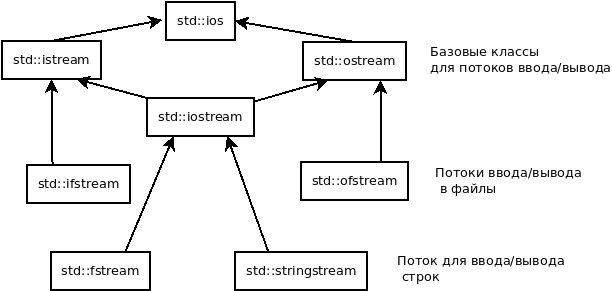
\includegraphics[width=0.8\textwidth]{io_classes.png}
\end{center}

Глобальные переенные \texttt{cin} (istream), \texttt{cout} (ostream), \texttt{cerr} (ostream).

Стандартная библиотека содержит перегруженные операторы \texttt{operator >>}, \texttt{operator <<} для примитивных типов и строк. 

\begin{minted}[fontsize=\footnotesize,numbersep=3pt,framesep=1mm,linenos,frame=single,label=]{cpp}
std::ostream& operator << (std::ostream& os, int v) {
    // convert int to bytes, write bytes
    return os;
}
\end{minted}
\begin{minted}[fontsize=\footnotesize,numbersep=3pt,framesep=1mm,linenos,frame=single,label=]{cpp}
std::istream& operator >> (std::istream& is, int& v) {
    // read bytes, convert to int
    return is;
}
\end{minted}
Такой код приводит к очистке буфера fflush потока, что замедляет вывод:
\begin{minted}[fontsize=\footnotesize,numbersep=3pt,framesep=1mm,linenos,frame=single,label=]{cpp}
std::cout << x << std::endl;
\end{minted}
Оператор читает строку до пробела, getline до конца строки:
\begin{minted}[fontsize=\footnotesize,numbersep=3pt,framesep=1mm,linenos,frame=single,label=]{cpp}
std::ifstream ifstream if("in.txt");
std::string word;
if >> word;
std::string line;
getline(if, line);
\end{minted}
Побайтовый ввод/вывод: read, write, seekg, tellg.

\subsection{Обработка ошибок}
rdstate() --- чем закончиласть последняя операция: eofbit, goodbit, failbit (считываем другим типом), badbit (не существует файла)
\subsection{Формат вывода}
\begin{minted}[fontsize=\footnotesize,numbersep=3pt,framesep=1mm,linenos,frame=single,label=]{cpp}
int x = 255;
std::cout.setf(std::ios::hex, std::ios::basefield);
std::cout << x; // после вывода флаг очистится
\end{minted}
Через манипуляторы
\begin{minted}[fontsize=\footnotesize,numbersep=3pt,framesep=1mm,linenos,frame=single,label=]{cpp}
ostream& operator << (ostream& (*pf)(ostream&));
\end{minted}
\subsection{Ввод-вывод пользовательских типов}
\begin{minted}[fontsize=\footnotesize,numbersep=3pt,framesep=1mm,linenos,frame=single,label=]{cpp}
class Point {
private:
    int x;
    int y;
public:
    friend ostream& operator << (ostream& os, const Point& p);
    friend istream& operator << (istream& is, Point& p);
    // friend функция может иметь доступ к приватным членам
};

ostream& operator << (ostream& os, const Point& p) {
    os << p.x << " " << p.y << "\n";
    return os;
}
istream& operator << (istream& is, Point& p) {
    is >> p.x >> p.y;
    return is;
}
\end{minted}
Так как ostream --- базовый класс, можно использовать один и тот же оператор для вывода на экран, строку и файл:
(cout, ofstream of("file"), stringstream ss).

